\documentclass{beamer}
\usetheme{Madrid}
\usecolortheme{beaver}
\usepackage{graphicx}
\graphicspath{ {pics} }
\usepackage{listings}
\usepackage{xcolor}
\usepackage{tikz}

\lstset{
    language=Python,
    basicstyle=\ttfamily\footnotesize,
    keywordstyle=\color{blue},
    commentstyle=\color{gray},
    stringstyle=\color{red},
    frame=single
}
%Information to be included in the title page:

\title{Understanding Computer Science}
\author{Nithin Vadekkapat}
\date{\today}

\begin{document}

\frame{\titlepage}

\begin{frame}{What is Computer Science?}
    \begin{itemize}
        \item Computer Science is not merely the study of computers.
        \item Computers are tools that aid in problem-solving.
        \item The focus is on problems, problem-solving, and algorithmic solutions.
    \end{itemize}
\end{frame}

\begin{frame}{The Role of Algorithms}
    \begin{itemize}
        \item An algorithm is a step-by-step set of instructions to solve a problem.
        \item Some problems may not have a solution.
        \item Computer Science studies both solvable and unsolvable problems.
    \end{itemize}
\end{frame}

\begin{frame}{Computability in Computer Science}
    \begin{itemize}
        \item A problem is \textbf{computable} if an algorithm exists to solve it.
        \item Computer Science studies both computable and non-computable problems.
        \item Solutions are independent of the machine used.
    \end{itemize}
\end{frame}

\begin{frame}{Abstraction in Computer Science}
    \begin{itemize}
        \item Abstraction helps separate the logical and physical perspectives.
        \item Example: Driving a car.
        \item Users interact with the interface without needing to understand the mechanics.
    \end{itemize}
\end{frame}

\begin{frame}[fragile]{Procedural Abstraction}
    \begin{itemize}
        \item Users (clients) do not need to know implementation details.
        \item The interface provides a way to interact with complex implementations.
        \item Example: Python's \texttt{math} module.
    \end{itemize}

    \vspace{0.5cm} % Adds space for better readability

    
    \begin{lstlisting}
import math
math.sqrt(16)
    \end{lstlisting}

    \vspace{0.5cm} % Adds space before continuing the list

    \begin{itemize}
        \item We do not need to know how \texttt{sqrt} is implemented.
        \item We only need to know its name and how to use it.
    \end{itemize}
\end{frame}

\begin{frame}{Programming and Algorithms}
    \begin{itemize}
        \item Programming is encoding an algorithm into a notation (programming language) for computer execution
        \item Without an algorithm, there can be no program
        \item Computer science is not just programming, but programming is an essential part
        \item Programming creates representations of our solutions
    \end{itemize}
\end{frame}

\begin{frame}{From Algorithms to Programs}
    \begin{itemize}
        \item Algorithms describe solutions in terms of:
        \begin{itemize}
            \item Data needed to represent the problem instance
            \item Steps necessary to produce the intended result
        \end{itemize}
        \item Programming languages must provide notation for both process and data
        \item Languages provide control constructs and data types
    \end{itemize}
\end{frame}

\begin{frame}{Control Constructs}
    \begin{itemize}
        \item Control constructs allow algorithmic steps to be represented unambiguously
        \item Minimum requirements for algorithm representation:
        \begin{itemize}
            \item Sequential processing
            \item Selection for decision-making
            \item Iteration for repetitive control
        \end{itemize}
        \item Any language with these basic statements can represent algorithms
    \end{itemize}
\end{frame}

\begin{frame}{Data Types}
    \begin{itemize}
        \item All data in computers are strings of binary digits
        \item Data types provide interpretation for binary data
        \item Built-in/primitive data types are building blocks for algorithm development
        \item Example: Integer data type
        \begin{itemize}
            \item Binary digits interpreted as familiar numbers (23, 654, -19)
            \item Supports operations like addition, subtraction, multiplication
        \end{itemize}
    \end{itemize}
\end{frame}

\begin{frame}{Complexity Challenges}
    \begin{itemize}
        \item Problems and solutions are often very complex
        \item Simple language-provided constructs and data types:
        \begin{itemize}
            \item Are sufficient to represent complex solutions
            \item But can be at a disadvantage during problem-solving
        \end{itemize}
        \item Higher-level abstractions help manage this complexity
    \end{itemize}
\end{frame}

\begin{frame}{Abstraction in Problem-Solving}
    \begin{itemize}
        \item Computer scientists use abstractions to focus on the "big picture"
        \item Creating models of the problem domain enables:
        \begin{itemize}
            \item More efficient problem-solving process
            \item More consistent description of data with respect to the problem
        \end{itemize}
        \item Abstractions allow us to ignore implementation details temporarily
    \end{itemize}
\end{frame}

\begin{frame}{Data Abstraction}
    \begin{itemize}
        \item Abstract Data Type (ADT): logical description of data and operations
        \item Focuses on \textit{what} the data represents, not \textit{how} it's constructed
        \item Creates encapsulation around data through information hiding
        \item Users interact with the interface only, not the implementation
    \end{itemize}
\end{frame}

\begin{frame}{ADT Implementation}
    \begin{itemize}
        \item Implementation of an ADT is called a data structure
        \item Data structure provides the physical view of the data
        \item Uses programming constructs and primitive data types
        \item Different implementations can satisfy the same ADT
        \item Choice of implementation affects efficiency
    \end{itemize}
\end{frame}



    

\begin{frame}{Python Data Structures}
    \begin{itemize}
        \item Python provides built-in data structures
        \item These structures are used to represent data in programs
        \item Common data structures include:
        \begin{itemize}
            \item Lists
            \item Tuples
            \item Sets
            \item Dictionaries
        \end{itemize}
    \end{itemize}
\end{frame}


\begin{frame}{Objects}
    \begin{itemize}
        \item Everything in Python is an object
        \item Objects have attributes and methods
        \item Objects can be created from classes
        \item Classes define the attributes and methods of objects
    \end{itemize}
\end{frame}
\begin{frame}
    \begin{figure}
        \centering
        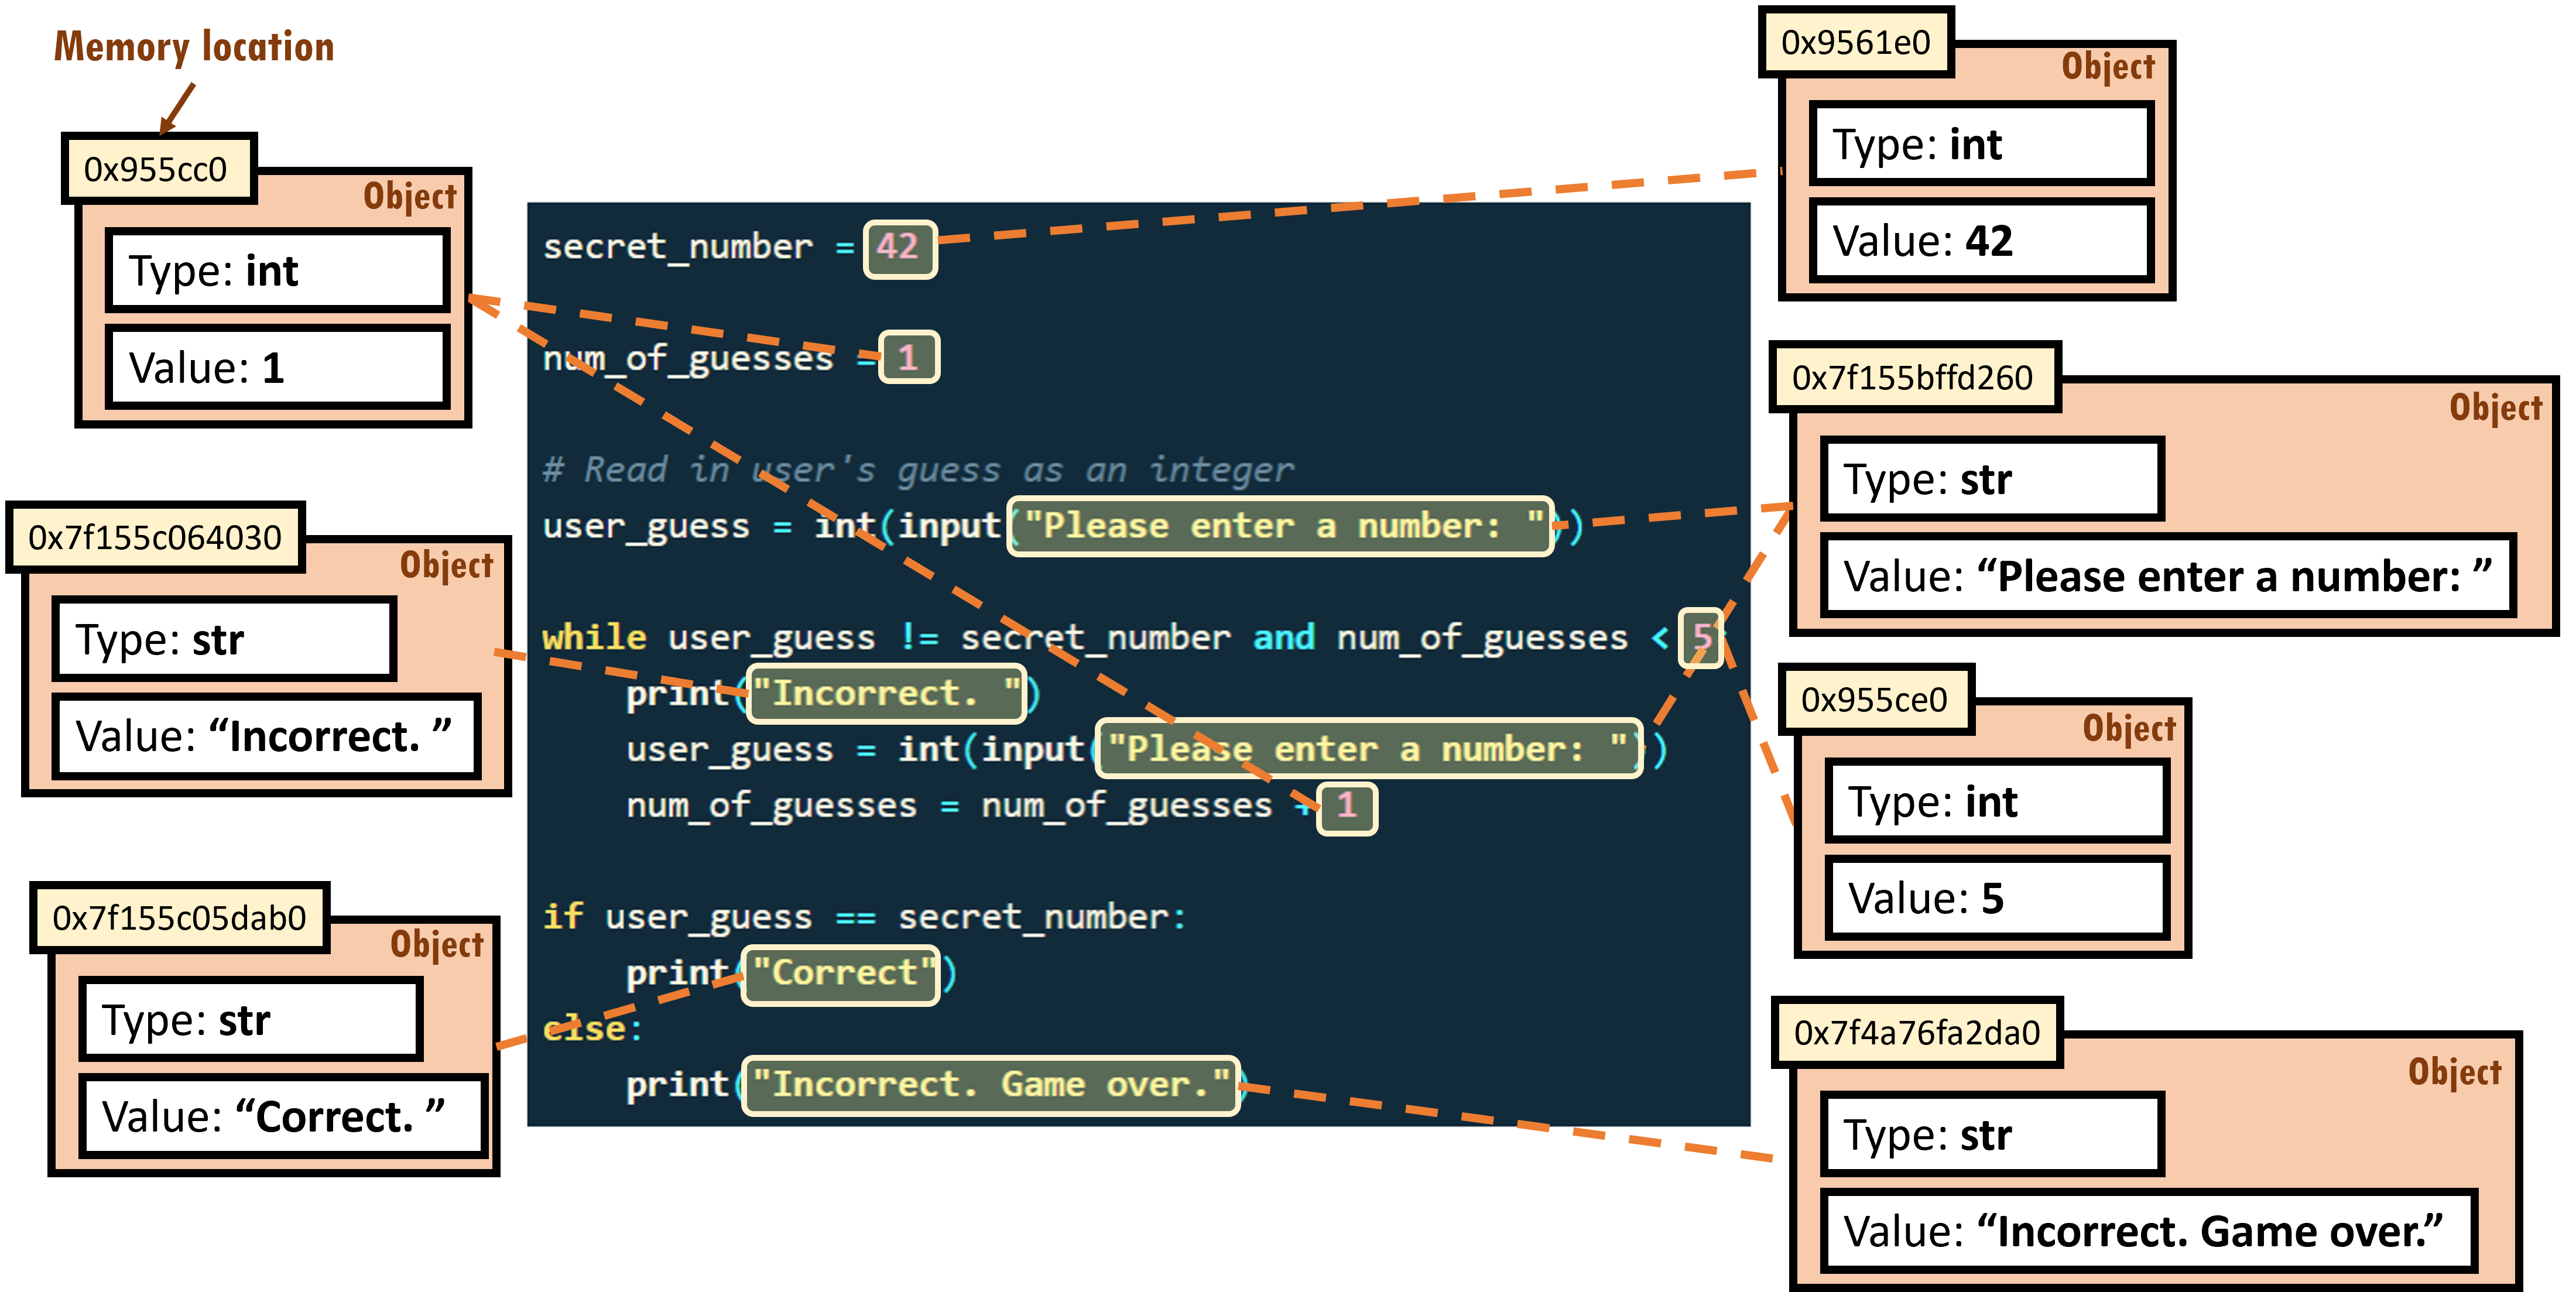
\includegraphics[width=1.0\textwidth]{pics/objects.png}
        \caption{Objects in Python}
    \end{figure}
\end{frame}

\section{Python Data Structures}
\begin{frame}{Built in atomic datatypes}
    \begin{itemize}
        \item Python provides built-in data types
        \item These types are used to represent data in programs
        \item Common data types include:
        \begin{itemize}
            \item Integers
            \item Floats
            \item Strings
            \item Booleans
        \end{itemize}
    \end{itemize}

\end{frame}

\begin{frame}{Operators and Expressions}
    \begin{columns}
        \column{0.5\textwidth}
        \begin{itemize}
            \item Objects can be combined using operators
            \item Arithmrtic operators in python 
            \begin{itemize}
            \item \texttt{+} (addition)
            \item \texttt{-} (subtraction)
            \item \texttt{*} (multiplication)
            \item \texttt{/} (division)
            \item \texttt{//} (floor division, or integer part of division)
            \item \texttt{\%} (modulo, or remainder after division)
            \item \texttt{**} (exponential - raised to the power)
            \end{itemize}
                    \end{itemize}
        \column{0.5\textwidth}
        \begin{figure}
            \centering
            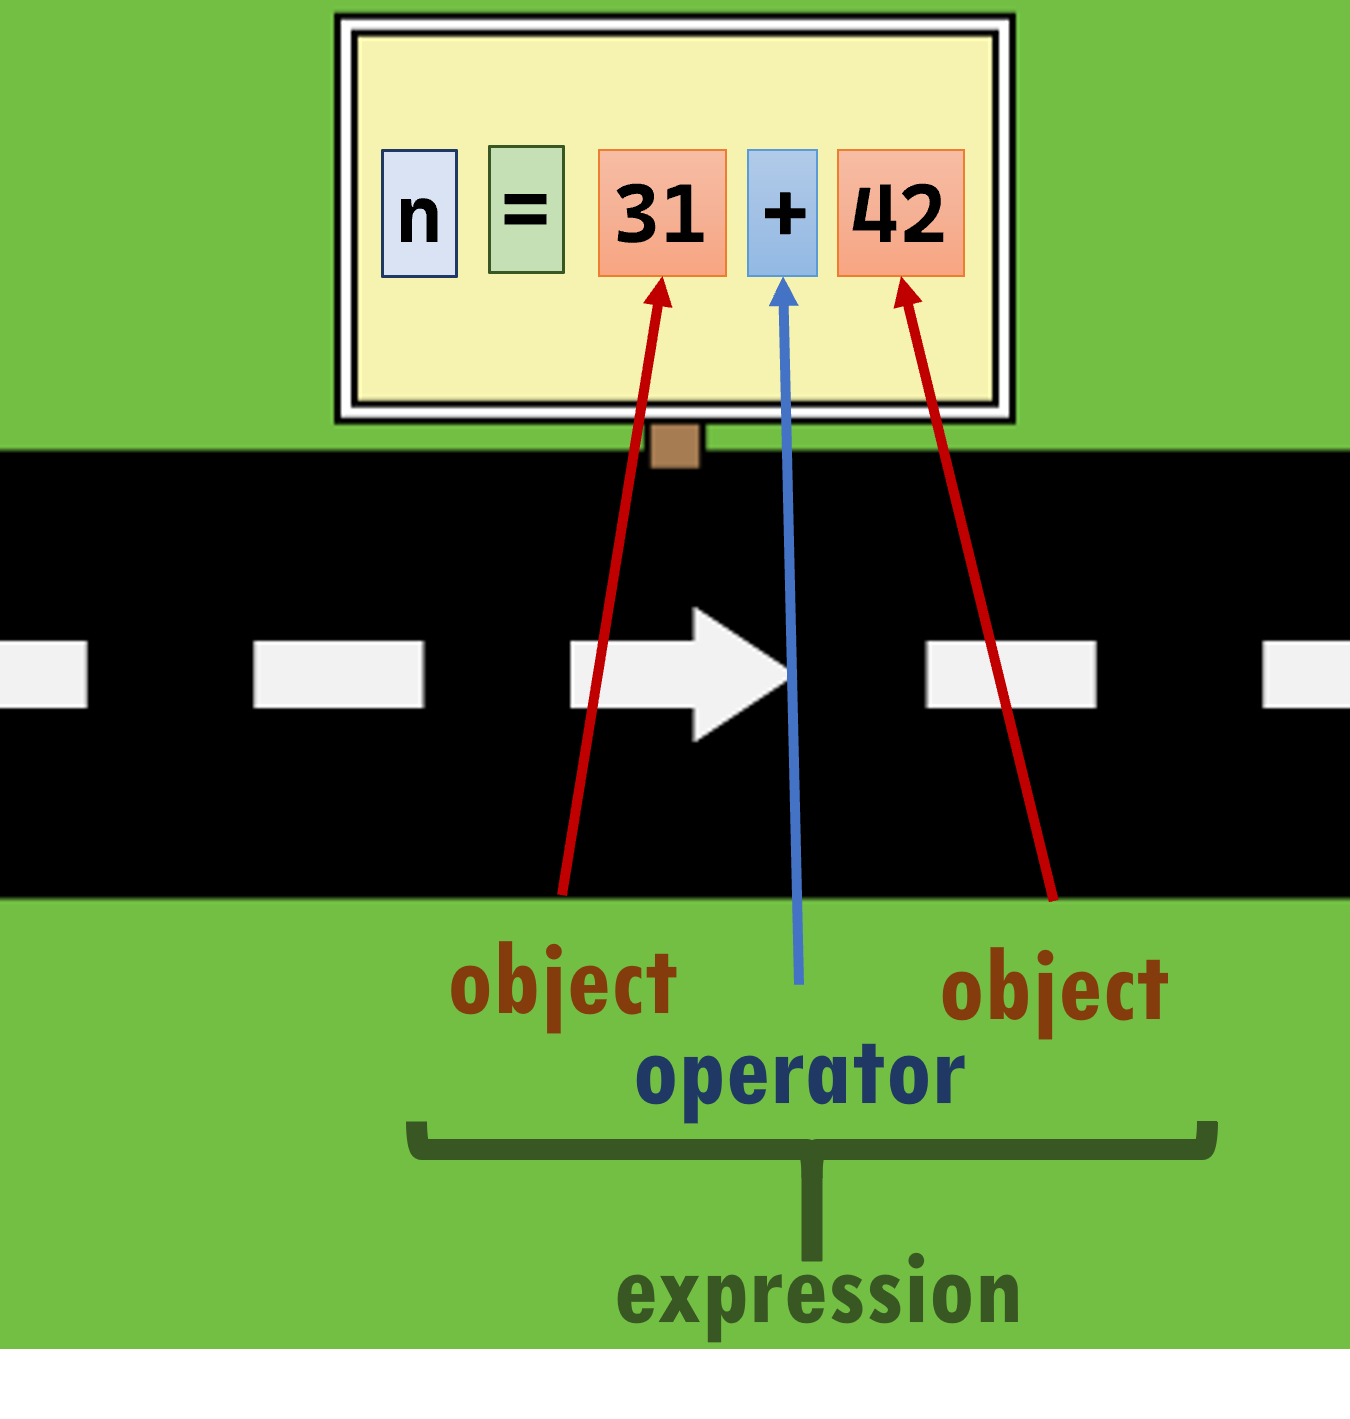
\includegraphics[width=0.8\textwidth]{pics/operator.png}
            \caption{Operators in Python}
        \end{figure}
    \end{columns}
\end{frame}
\begin{frame}{Python Operator Precedence}
    \begin{itemize}
        \item Python evaluates expressions based on operator precedence.
        \item Common operators in order of precedence (from highest to lowest):
        \begin{itemize}
            \item \texttt{()} - Parentheses
            \item \texttt{**} - Exponentiation
            \item \texttt{+x}, \texttt{-x}, \texttt{\textasciitilde{}x} - Unary plus, Unary minus, Bitwise NOT
            \item \texttt{*}, \texttt{/}, \texttt{//}, \texttt{\%} - Multiplication, Division, Floor division, Modulus
            \item \texttt{+}, \texttt{-} - Addition, Subtraction
            \item \texttt{<<}, \texttt{>>} - Bitwise shift operators
            \item \texttt{\&} - Bitwise AND
            \item \texttt{\textasciicircum} - Bitwise XOR
            \item \texttt{|} - Bitwise OR
            \item \texttt{==}, \texttt{!=}, \texttt{>}, \texttt{<}, \texttt{>=}, \texttt{<=}, \texttt{is}, \texttt{is not}, \texttt{in}, \texttt{not in} - Comparisons, Identity, Membership
            \item \texttt{not} - Logical NOT
            \item \texttt{and} - Logical AND
            \item \texttt{or} - Logical OR
        \end{itemize}
        \item Example: \texttt{1 + 2 * 3 == 7} evaluates as \texttt{1 + (2 * 3) == 7}, which is \texttt{1 + 6 == 7}, resulting in \texttt{True}.
    \end{itemize}
\end{frame}
\begin{frame}[fragile]{Overloaded Operators}
    \begin{itemize}
        \item Some operators are not limited to arithmetic operations with numbers.
        \item For example, \texttt{+} and \texttt{*} can be used for a different kind of operation when used with strings.
    \end{itemize}
    \begin{lstlisting}{python}
>>> 'hello' + 'world'
'helloworld'
>>> 'hello' * 3
'hellohellohello'
    \end{lstlisting}
\end{frame}

\begin{frame}{Variables}
    In Python, a variable is simply a name or a label that points to an object instance in memory
    \begin{figure}
        \centering
        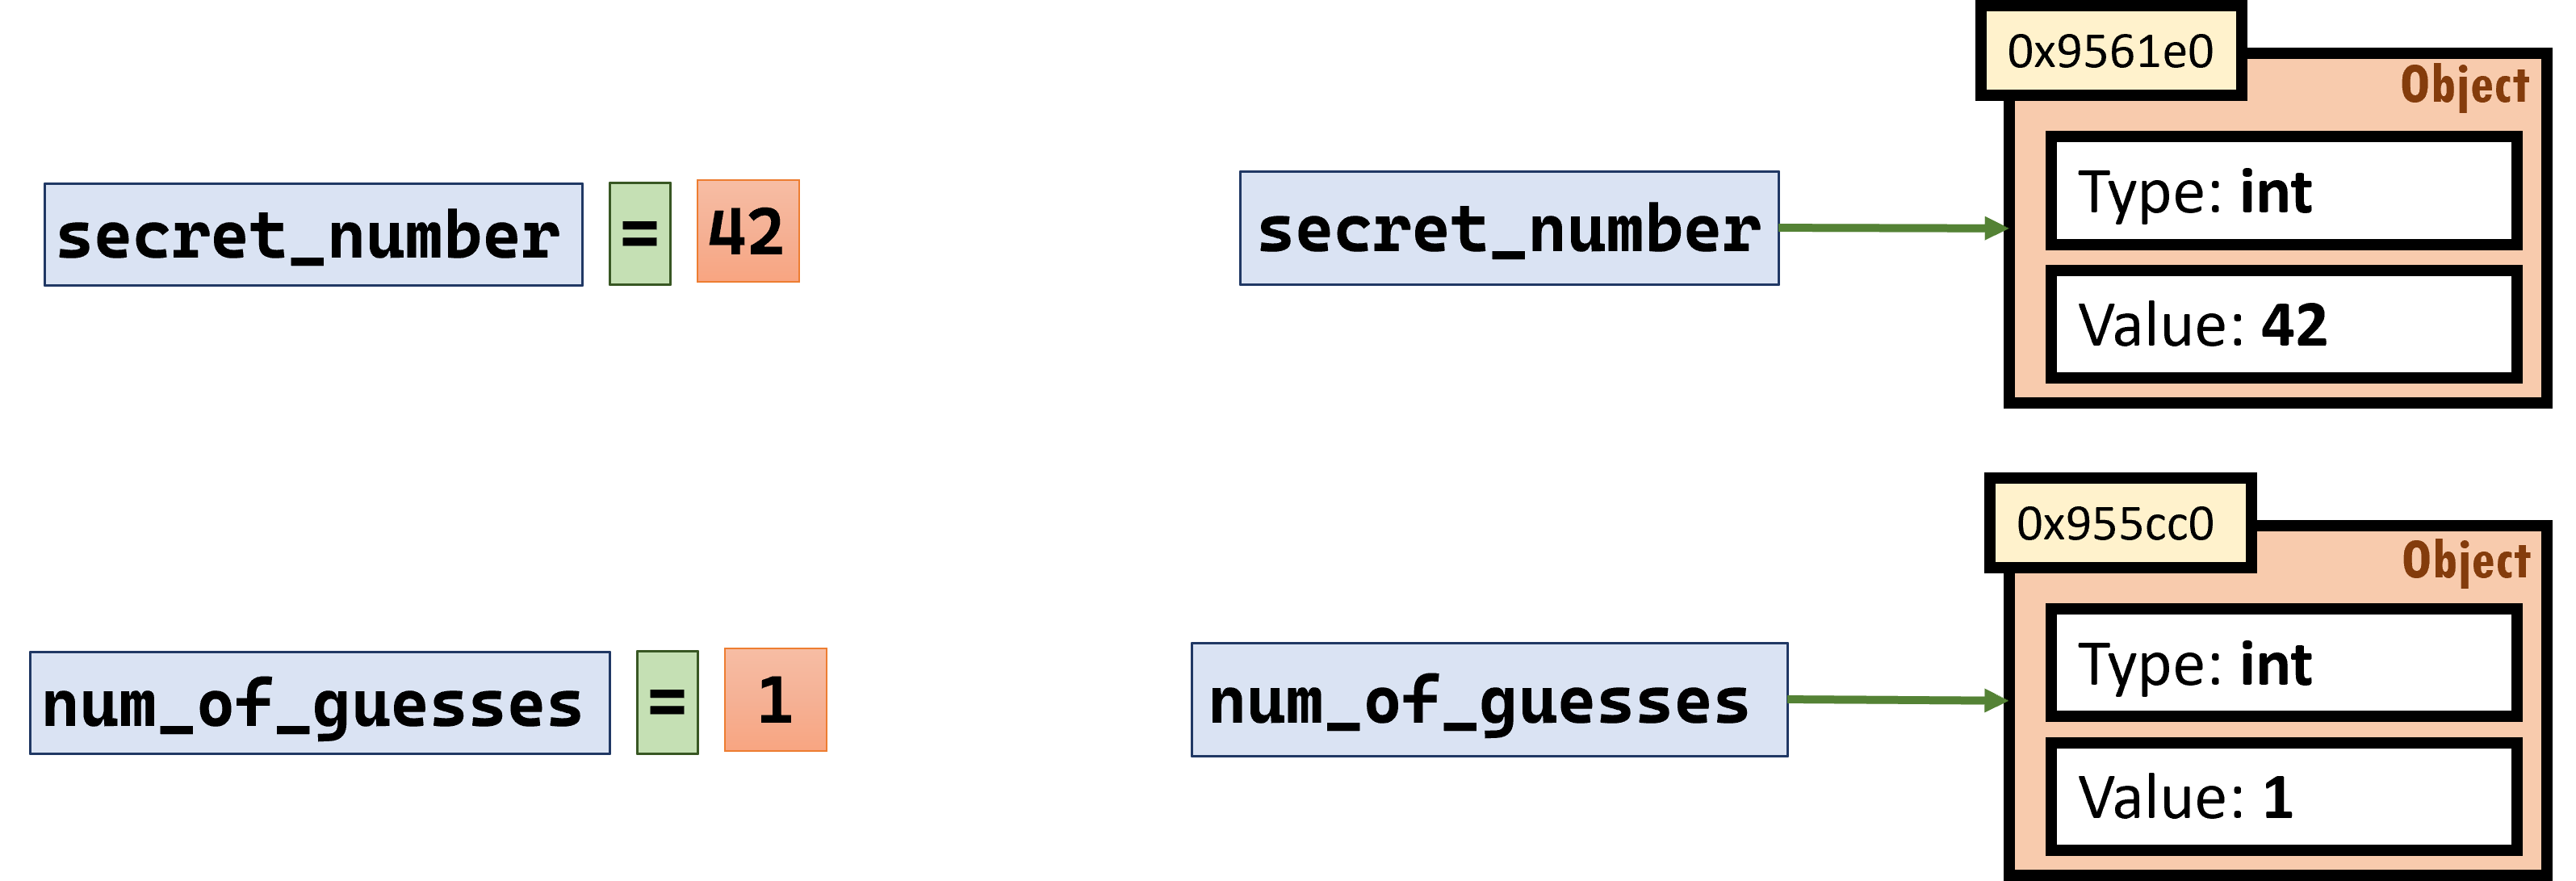
\includegraphics[width=0.8\textwidth]{pics/variable.png}
        \caption{Variables in Python}
    \end{figure}
\end{frame}

\begin{frame}{Variable Assignments}
    \begin{columns}
        \column{0.5\textwidth}
        \begin{figure}
            \centering
            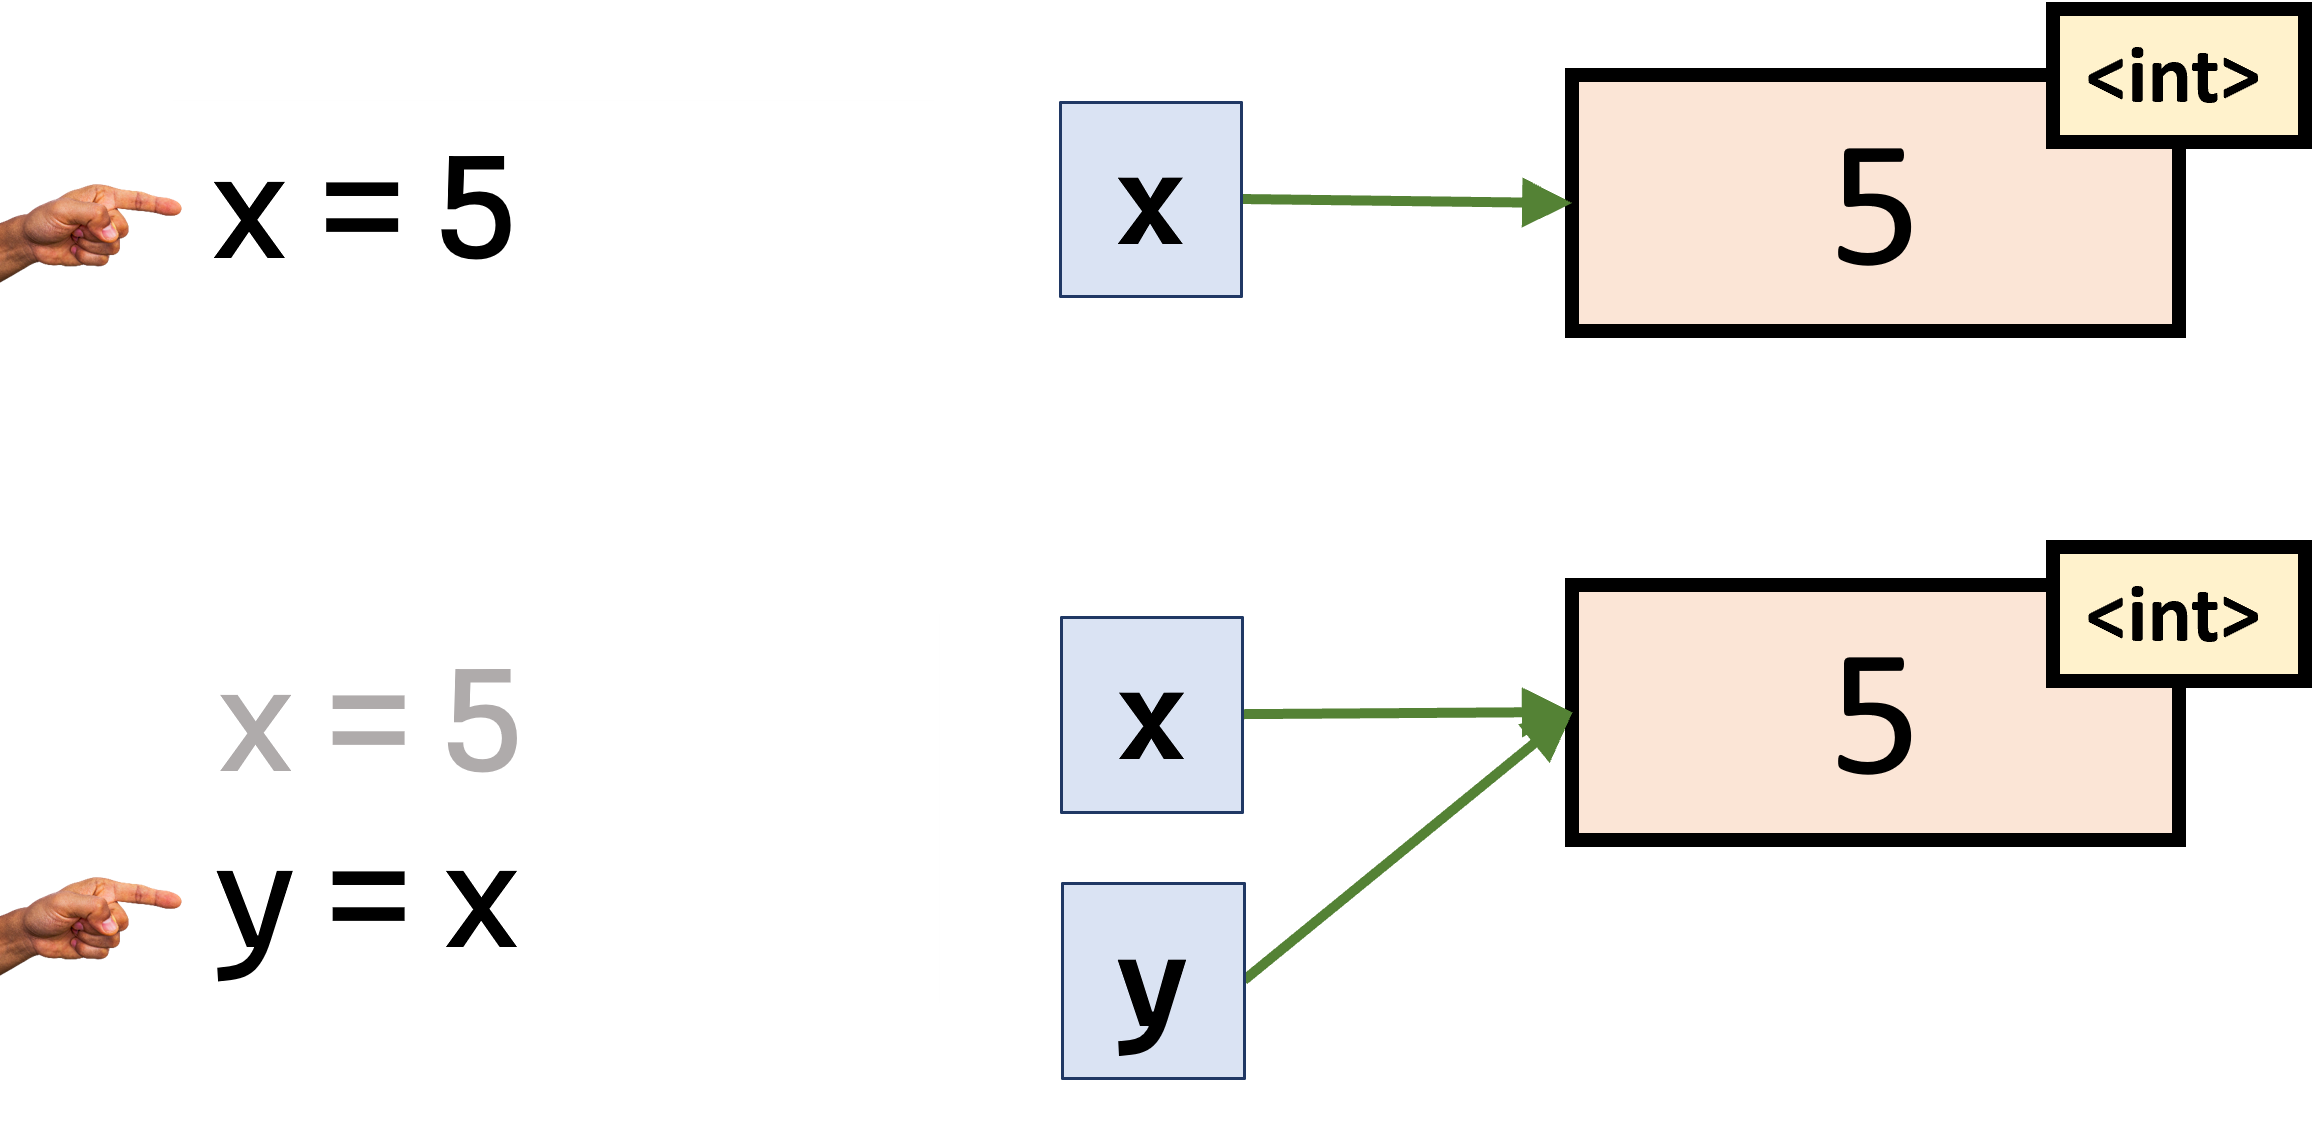
\includegraphics[width=0.8\textwidth]{pics/assignment.png}
            \caption{Variable Assignment}
        \end{figure}
        \column{0.5\textwidth}
        \begin{figure}
            \centering
            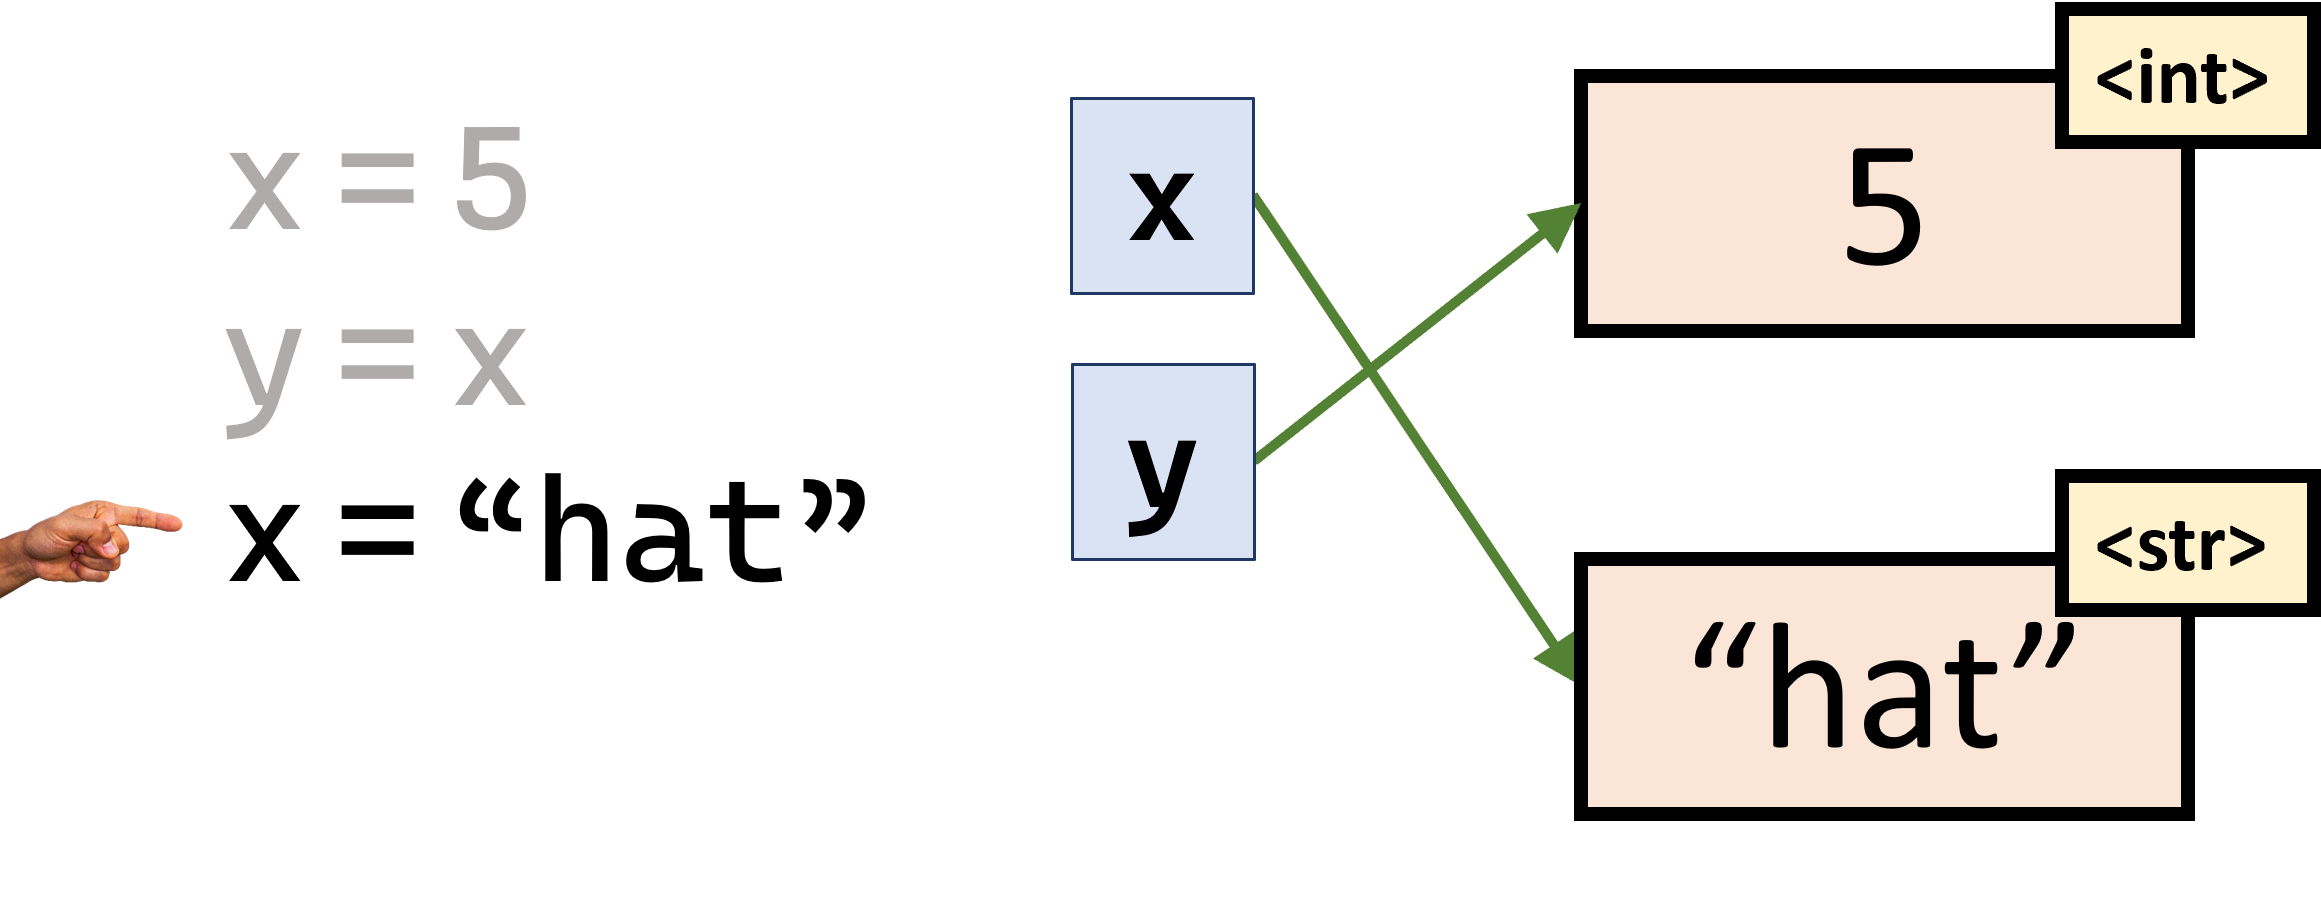
\includegraphics[width=0.8\textwidth]{pics/assignment2.png}
            \caption{Variable Assignment}
        \end{figure}
    \end{columns}
    
\end{frame}

\begin{frame}[fragile]{Variable Assignment}
    \begin{lstlisting}{python}
>>> x = 20
>>> y = x
>>> x = "hello"
>>> print(y)
20
>>> print(x)
hello
    \end{lstlisting}
\end{frame}


\begin{frame}{Naming Variables}
    \begin{itemize}
        \item Variable names must start with a letter or an underscore
        \item The rest of the name can contain letters, numbers, and underscores
        \item Variable names are case-sensitive
        \item Variable names should be descriptive
    \end{itemize}
\end{frame}

\begin{frame}[fragile]{Reserved Keywords}
    \begin{lstlisting}{Python}
     >>> import keyword
     >>> keyword.kwlist      
    \end{lstlisting}
\end{frame} 

\begin{frame}
    \frametitle{Comparison Operators}
    \begin{itemize}
        \item Comparison operators are used to compare two values
        \item They return a boolean value (True or False)
        \item Common comparison operators include:
        \begin{itemize}
            \item \texttt{==} (equal to)
            \item \texttt{!=} (not equal to)
            \item \texttt{>} (greater than)
            \item \texttt{<} (less than)
            \item \texttt{>=} (greater than or equal to)
            \item \texttt{<=} (less than or equal to)
        \end{itemize}
    \end{itemize}
\end{frame}


\begin{frame}[fragile]{Python Quiz-1}
\begin{lstlisting}{Python}
>>> 5 == 5.0000
>>> 1+2 == 3 
>>> 9 > 8.999999999999999
>>> 6 // 3 == 6.0 / 3.0
\end{lstlisting}
\end{frame}

\begin{frame}[fragile]{Floating-Point Comparisons}
    \begin{itemize}
        \item Floating-point numbers can have precision issues due to their representation in memory.
        \item Comparisons involving equality can be affected by these precision issues.
        \item Example: \texttt{1.1 + 2.2 == 3.3} evaluates to \texttt{False} due to tiny inaccuracies.
        \item However, comparisons involving inequality are less likely to be affected.
        \item Example: \texttt{9 > 8.999999999999999} evaluates to \texttt{True}.
    \end{itemize}
    \begin{lstlisting}{python}
>>> 1.1 + 2.2 == 3.3
False
>>> 9 > 8.999999999999999
True
    \end{lstlisting}
\end{frame}

\begin{frame}[fragile]
    \frametitle{Python Quiz-2}
    \begin{lstlisting}{Python}
>>> 5 != 5.0000
>>> True != False
>>> False < True
>>> "10" > "2"
    \end{lstlisting}
\end{frame}

\begin{frame}[fragile]{String Comparison}
    \begin{itemize}
        \item When comparing two strings, Python compares the "Unicode code point" of the first character of each string.
        \item If the first characters are the same, it compares the second characters, and so on, until one of the strings ends
    \end{itemize}
    \begin{lstlisting}{python}
>>> "10" > "2"
False
>>> ord("1")
49
>>> ord("2")
50
    \end{lstlisting}
    \begin{itemize}
        \item This explains why files on your computer might be sorted in this order:
        \begin{itemize}
            \item \texttt{"Picture1.jpg"}
            \item \texttt{"Picture10.jpg"}
            \item \texttt{"Picture100.jpg"}
            \item \texttt{"Picture11.jpg"}
            \item \texttt{"Picture2.jpg"}
        \end{itemize}
    \end{itemize}
\end{frame}


\begin{frame}[fragile]{Naming Your Robot}
    \begin{itemize}
        \item Use \texttt{input()} to read the robot's name from the user.
        \item Assign the name to a variable called \texttt{name}.
        \item Assign an identifier to the robot, e.g., \texttt{identifier = 1000}.
        \item Print a message from the robot using \texttt{print()}.
    \end{itemize}
    \begin{lstlisting}{Python}
>>> name = input("Enter the robot's name: ")
>>> identifier = 1000
>>> print(f"Hello. My name is {name}. My ID is {identifier}.")
    \end{lstlisting}
\end{frame}

\begin{frame}[fragile]{Converting 2D Index to 1D Index}
    \begin{itemize}
        \item User provides the number of rows \(R\), number of columns \(C\), and a 2D index \((r, c)\)
        \item Convert the 2D index \((r, c)\) to a 1D index \(s\) using row-major ordering.
    \end{itemize}
    \begin{lstlisting}{python}
# Get user input
R = int(input("Enter the number of rows: "))
C = int(input("Enter the number of columns: "))
r = int(input("Enter the row index: "))
c = int(input("Enter the column index: "))
s = r*R + c
# Print the result
print(f"The 1D index is: {s}")
    \end{lstlisting}
\end{frame}



\end{document}
